\clearpage
\section{Discussion}
\todo[inline]{how to handle suboptimally solved instances}

\subsection{FBA and ll-FBA Variants}
\begin{figure}[h!]
    \caption{performance of ll-FBA variants}
    \centering
    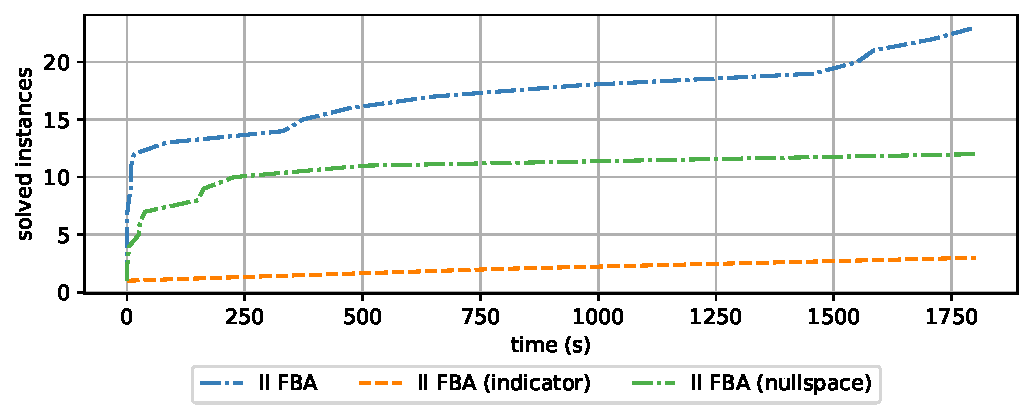
\includegraphics[width=1.0\textwidth]{Images/fba_variants_comparison_plot.pdf}
    \label{fig:ll_fba_comparion}
    \subcaption*{The results are shown in \cref{tab:ll_fba_comparison} and in \cref{tab:ll_fba_indicator}}
\end{figure}

% \begin{table}[!ht]
%     \centering
%     \begin{tabular}{|l|l|l|l|l|l|l|l|}
%     \hline
%         \thead{organism} & \thead{type} & \thead{objective} & \thead{dual bound} & \thead{termination} & \thead{time limit} & \thead{time (s)} & \thead{nodes} \\ \hline
%         iAF692 & loopless\_fba & 0.0268 & 0.0268 & OPTIMAL & 1800 & 4.51 & 351 \\ \hline
%         iAF692 & loopless\_fba\_nullspace & 0.0256 & 0.0268 & TIME\_LIMIT & 1800 & 1800.0 & 575 \\ \hline
%         iAF692 & loopless\_indicator\_fba & 0.0268 & 0.0268 & OPTIMAL & 1800 & 1285.4 & 11532 \\ \hline
%         iJR904 & loopless\_fba & 0.9219 & 0.9219 & OPTIMAL & 1800 & 114.67 & 7614 \\ \hline
%         iJR904 & loopless\_fba\_nullspace & 0.9219 & 0.9219 & OPTIMAL & 1800 & 172.86 & 641 \\ \hline
%         iJR904 & loopless\_indicator\_fba & 0.0 & 0.9219 & TIME\_LIMIT & 1800 & 1800.0 & 31243 \\ \hline
%         iML1515 & loopless\_fba & 0.865 & 0.877 & TIME\_LIMIT & 1800 & 1800.0 & 12098 \\ \hline
%         iML1515 & loopless\_fba\_nullspace & NaN & NaN & TIME\_LIMIT & 1800 & 1800.06 & 15 \\ \hline
%         iML1515 & loopless\_indicator\_fba & NaN & NaN & TIME\_LIMIT & 1800 & 1800.38 & 6776 \\ \hline
%     \end{tabular}
% \end{table}

\subsection{Blocking Cycles in FBA}
\begin{figure}[h!]
    \caption{runtime of ll-FBA and ll-FBA with blocked cycles}
    \centering
    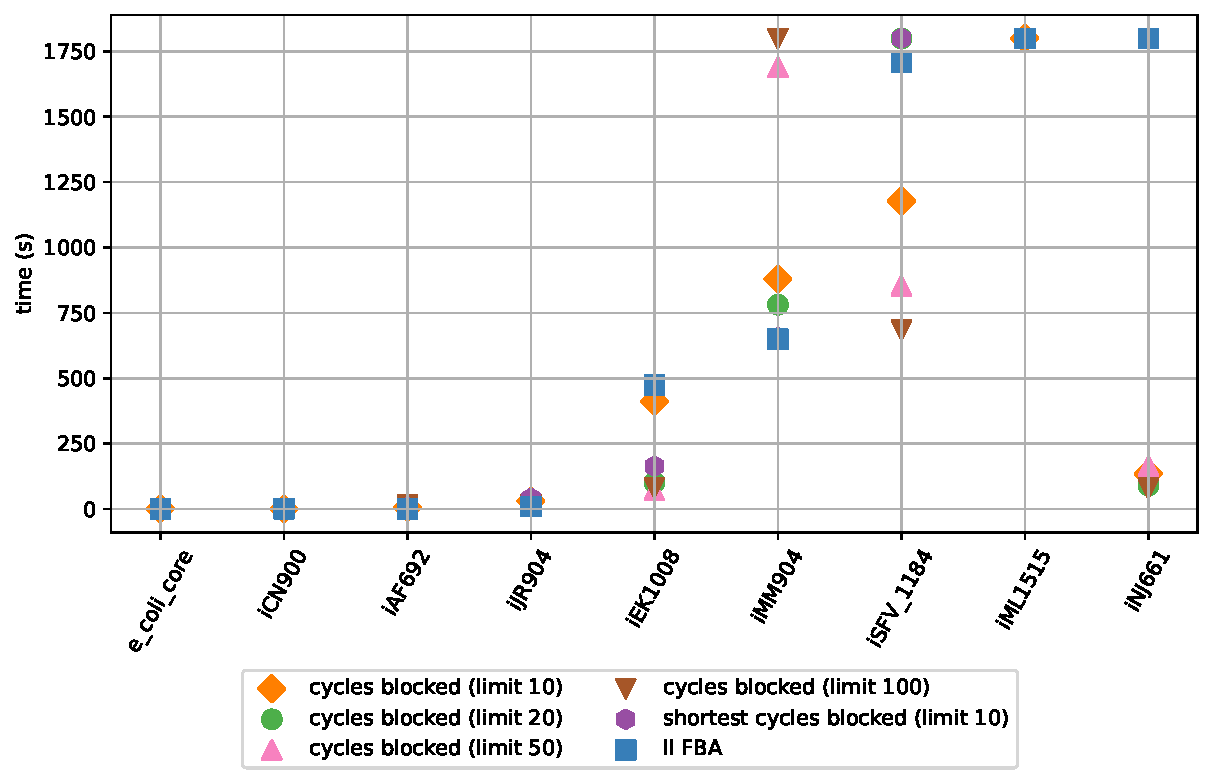
\includegraphics[width=1.0\textwidth]{Images/cff_comparison.pdf}
    \label{fig:cff_comparison}
    \subcaption*{The results are shown in \cref{tab:cff} and \cref{tab:cff_shortest_cycles}}
\end{figure}

% \begin{table}[!ht]
%     \centering
%     \begin{tabular}{|l|l|l|l|l|l|}
%     \hline
%     \thead{\textbf{iAF692}} & \thead{objective} & \thead{status} & \thead{blocked cycles} & \thead{time (s)} & \thead{nodes} \\ \hline
%         loopless\_fba\_blocked & 0.0268 & OPTIMAL & 50 & 7.33 & 1699 \\ \hline
%         loopless\_fba\_blocked & 0.0268 & OPTIMAL & 100 & 6.51 & 818 \\ \hline
%         loopless\_fba\_blocked\_shortest\_cycles & 0.0268 & OPTIMAL & 50 & 7.34 & 1528 \\ \hline
%         loopless\_fba\_blocked\_shortest\_cycles & 0.0268 & OPTIMAL & 100 & 6.39 & 917 \\ \hline
%     \end{tabular}
% \end{table}

% \begin{table}[!ht]
%     \centering
%     \begin{tabular}{|l|l|l|l|l|l|}
%     \hline
%     \thead{\textbf{iJR904}} & \thead{objective} & \thead{status} & \thead{blocked cycles} & \thead{time (s)} & \thead{nodes} \\ \hline
%         loopless\_fba\_blocked & 0.9219 & OPTIMAL & 50 & 92.41 & 6505 \\ \hline
%         loopless\_fba\_blocked & 0.9219 & OPTIMAL & 100 & 48.27 & 2314 \\ \hline
%         loopless\_fba\_blocked\_shortest\_cycles & 0.9219 & OPTIMAL & 50 & 73.95 & 5777 \\ \hline
%         loopless\_fba\_blocked\_shortest\_cycles & 0.9219 & OPTIMAL & 100 & 30.22 & 365 \\ \hline
%     \end{tabular}
% \end{table}

% \begin{sidewaystable}
%     \begin{tabular}{|l|l|l|l|l|l|l|l|l|}
%     \hline
%         \thead{\textbf{iAF692}} & \thead{objective} & \thead{dual} & \thead{status} & \thead{blocked cycles} & \thead{ceiling} & \thead{block limit} & \thead{time (s)} & \thead{nodes} \\ \hline
%         loopless\_fba & 0.0268 & 0.0268 & OPTIMAL & ~ & ~ & ~ & 4.51 & 351 \\ \hline
%         loopless\_fba\_nullspace & 0.0256 & 0.0268 & TIME\_LIMIT & ~ & ~ & ~ & 1800.0 & 575 \\ \hline
%         loopless\_indicator\_fba & 0.0268 & 0.0268 & OPTIMAL & ~ & ~ & ~ & 1285.4 & 11532 \\ \hline
%         loopless\_indicator\_fba\_blocked\_same\_objective & 0.0268 & 0.0268 & OPTIMAL & 0 & 50 & 500 & 1286.58 & 11532 \\ \hline
%         loopless\_indicator\_fba\_blocked\_same\_objective & 0.0268 & 0.0268 & OPTIMAL & 0 & 100 & 500 & 1269.63 & 11532 \\ \hline
%         loopless\_fba\_blocked\_same\_objective & 0.0268 & 0.0268 & OPTIMAL & 0 & 50 & 100 & 4.53 & 351 \\ \hline
%         loopless\_fba\_blocked\_same\_objective & 0.0268 & 0.0268 & OPTIMAL & 0 & 100 & 100 & 4.51 & 351 \\ \hline
%         loopless\_fba\_blocked\_same\_objective & 0.0268 & 0.0268 & OPTIMAL & 0 & 200 & 100 & 4.51 & 351 \\ \hline
%         loopless\_fba\_blocked\_same\_objective & 0.0268 & 0.0268 & OPTIMAL & 0 & 500 & 100 & 4.5 & 351 \\ \hline
%         loopless\_fba\_blocked & 0.0268 & 0.0268 & OPTIMAL & 7 & 50 & 100 & 6.08 & 949 \\ \hline
%         loopless\_fba\_blocked & 0.0268 & 0.0268 & OPTIMAL & 7 & 100 & 100 & 6.09 & 949 \\ \hline
%         loopless\_fba\_blocked & 0.0268 & 0.0268 & OPTIMAL & 7 & 200 & 100 & 6.1 & 949 \\ \hline
%         loopless\_fba\_blocked & 0.0268 & 0.0268 & OPTIMAL & 7 & 500 & 100 & 6.07 & 949 \\ \hline
%         loopless\_fba\_blocked00 & 0.0268 & 0.0268 & OPTIMAL & 50 & 10000 & 50 & 7.34 & 1699 \\ \hline
%         loopless\_fba\_blocked00 & 0.0268 & 0.0268 & OPTIMAL & 100 & 10000 & 100 & 6.49 & 818 \\ \hline
%         loopless\_fba\_blocked\_shortest\_cycles00 & 0.0268 & 0.0268 & OPTIMAL & 50 & 10000 & 50 & 7.76 & 1528 \\ \hline
%         loopless\_fba\_blocked\_shortest\_cycles00 & 0.0268 & 0.0268 & OPTIMAL & 100 & 10000 & 100 & 6.38 & 917 \\ \hline
%     \end{tabular}


%     \vspace{5mm}

%     \begin{tabular}{|l|l|l|l|l|l|l|l|l|l|}
%     \hline
%         \thead{\textbf{iJR904}} & \thead{objective} & \thead{dual} & \thead{status} & \thead{blocked cycles} & \thead{ceiling} & \thead{block limit} & \thead{time (s)} & \thead{nodes} \\ \hline
%         loopless\_fba & 0.9219 & 0.9219 & OPTIMAL & ~ & ~ & ~ & 114.67 & 7614 \\ \hline
%         loopless\_fba\_nullspace & 0.9219 & 0.9219 & OPTIMAL & ~ & ~ & ~ & 172.86 & 641 \\ \hline
%         loopless\_indicator\_fba & 0.0 & 0.9219 & TIME\_LIMIT & ~ & ~ & ~ & 1800.0 & 31243 \\ \hline
%         loopless\_indicator\_fba\_blocked\_same\_objective & 0.0 & 0.9219 & TIME\_LIMIT & 0 & 50 & 500 & 1800.0 & 28423 \\ \hline
%         loopless\_indicator\_fba\_blocked\_same\_objective & 0.0 & 0.9219 & TIME\_LIMIT & 0 & 100 & 500 & 1800.0 & 28283 \\ \hline
%         loopless\_fba\_blocked\_same\_objective & 0.9219 & 0.9219 & OPTIMAL & 0 & 50 & 100 & 115.01 & 7614 \\ \hline
%         loopless\_fba\_blocked\_same\_objective & 0.9219 & 0.9219 & OPTIMAL & 0 & 100 & 100 & 114.7 & 7614 \\ \hline
%         loopless\_fba\_blocked\_same\_objective & 0.9219 & 0.9219 & OPTIMAL & 0 & 200 & 100 & 114.14 & 7614 \\ \hline
%         loopless\_fba\_blocked\_same\_objective & 0.9219 & 0.9219 & OPTIMAL & 0 & 500 & 100 & 110.62 & 7614 \\ \hline
%         loopless\_fba\_blocked & 0.9219 & 0.9219 & OPTIMAL & 13 & 50 & 100 & 89.4 & 4804 \\ \hline
%         loopless\_fba\_blocked & 0.9219 & 0.9219 & OPTIMAL & 20 & 100 & 100 & 45.61 & 881 \\ \hline
%         loopless\_fba\_blocked & 0.9219 & 0.9219 & OPTIMAL & 60 & 200 & 100 & 101.19 & 28 \\ \hline
%         loopless\_fba\_blocked & 0.9219 & 0.9219 & OPTIMAL & 100 & 500 & 100 & 48.43 & 2314 \\ \hline
%         loopless\_fba\_blocked00 & 0.9219 & 0.9219 & OPTIMAL & 50 & 10000 & 50 & 99.55 & 6505 \\ \hline
%         loopless\_fba\_blocked00 & 0.9219 & 0.9219 & OPTIMAL & 100 & 10000 & 100 & 48.28 & 2314 \\ \hline
%         loopless\_fba\_blocked\_shortest\_cycles00 & 0.9219 & 0.9219 & OPTIMAL & 50 & 10000 & 50 & 74.12 & 5777 \\ \hline
%         loopless\_fba\_blocked\_shortest\_cycles & 0.9219 & 0.9219 & OPTIMAL & 13 & 50 & 100 & 87.25 & 2792 \\ \hline
%     \end{tabular}
% \end{sidewaystable}

% \begin{sidewaystable}
%     \centering
%     \begin{tabular}{|l|l|l|l|l|l|l|l|l|}
%     \hline
%         \thead{\textbf{iML1515}} & \thead{objective} & \thead{dual} & \thead{status} & \thead{blocked cycles} & \thead{ceiling} & \thead{block limit} & \thead{time (s)} & \thead{nodes} \\ \hline
%        loopless\_fba & 0.865 & 0.877 & TIME\_LIMIT & ~ & ~ & ~ & 1800.0 & 12098 \\ \hline
%         loopless\_fba\_nullspace & NaN & NaN & TIME\_LIMIT & ~ & ~ & ~ & 1800.06 & 15 \\ \hline
%         loopless\_indicator\_fba & NaN & NaN & TIME\_LIMIT & ~ & ~ & ~ & 1800.38 & 6776 \\ \hline
%         loopless\_indicator\_fba\_blocked\_same\_objective & NaN & NaN & TIME\_LIMIT & 50 & 50 & 500 & 1800.0 & 8902 \\ \hline
%         loopless\_indicator\_fba\_blocked\_same\_objective & NaN & NaN & TIME\_LIMIT & 100 & 100 & 500 & 1800.56 & 6828 \\ \hline
%         loopless\_fba\_blocked\_same\_objective & 0.0 & 0.877 & TIME\_LIMIT & 50 & 50 & 100 & 1800.0 & 41468 \\ \hline
%         loopless\_fba\_blocked\_same\_objective & 0.0 & 0.877 & TIME\_LIMIT & 100 & 100 & 100 & 1800.0 & 51433 \\ \hline
%         loopless\_fba\_blocked\_same\_objective & 0.0 & 0.877 & TIME\_LIMIT & 100 & 200 & 100 & 1800.0 & 52372 \\ \hline
%         loopless\_fba\_blocked\_same\_objective & 0.0 & 0.877 & TIME\_LIMIT & 100 & 500 & 100 & 1800.05 & 52039 \\ \hline
%         loopless\_fba\_blocked & 0.0 & 0.877 & TIME\_LIMIT & 50 & 50 & 100 & 1800.0 & 45557 \\ \hline
%         loopless\_fba\_blocked & 0.0 & 0.877 & TIME\_LIMIT & 100 & 100 & 100 & 1800.0 & 41023 \\ \hline
%         loopless\_fba\_blocked & 0.0 & 0.877 & TIME\_LIMIT & 100 & 200 & 100 & 1800.0 & 40683 \\ \hline
%         loopless\_fba\_blocked & 0.0 & 0.877 & TIME\_LIMIT & 100 & 500 & 100 & 1800.0 & 40864 \\ \hline
%         loopless\_fba\_blocked\_shortest\_cycles & 0.2277 & 0.877 & TIME\_LIMIT & 50 & 50 & 100 & 1800.04 & 48769 \\ \hline
%     \end{tabular}
% \end{sidewaystable}

\subsection{No-Good Cuts}
\begin{figure}[h!]
    \caption{runtime of ll-FBA and ll-FBA with no-good cuts}
    \centering
    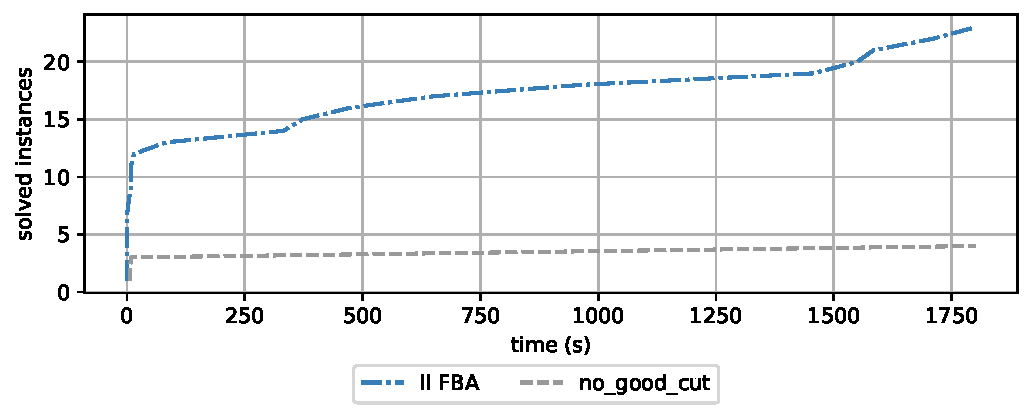
\includegraphics[width=1.0\textwidth]{Images/no_good_cuts_comparison_plot.pdf}
    \label{fig:cff_comparison}
    \subcaption*{The results are shown in \cref{tab:no_good_cuts}}
\end{figure}

\subsection{Combinatorial Benders' Cuts}

\begin{figure}[h!]
    \caption{solved instances by CB (indicator) and ll-FBA}
    \centering
    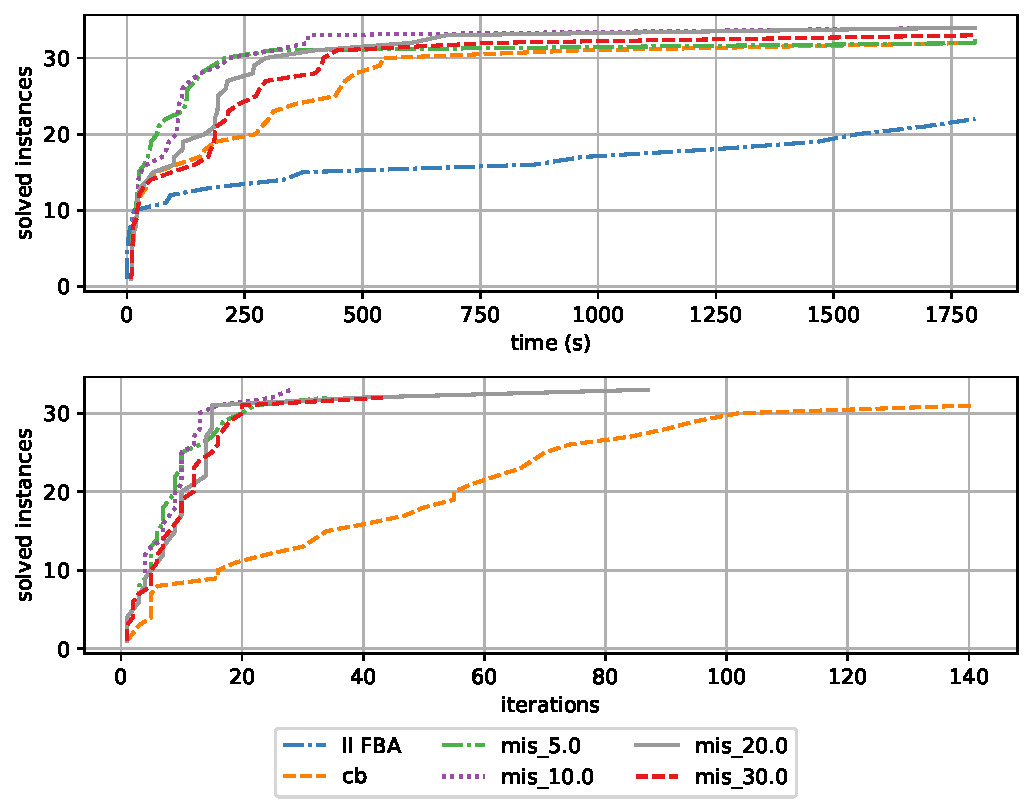
\includegraphics[width=0.8\textwidth]{Images/mis_comparison_solved_instances.pdf}
    \label{fig:mis_comparison_solved_instances}
\end{figure}

\begin{figure}[h!]
    \caption{solved instances by CB (indicator) and ll-FBA}
    \centering
    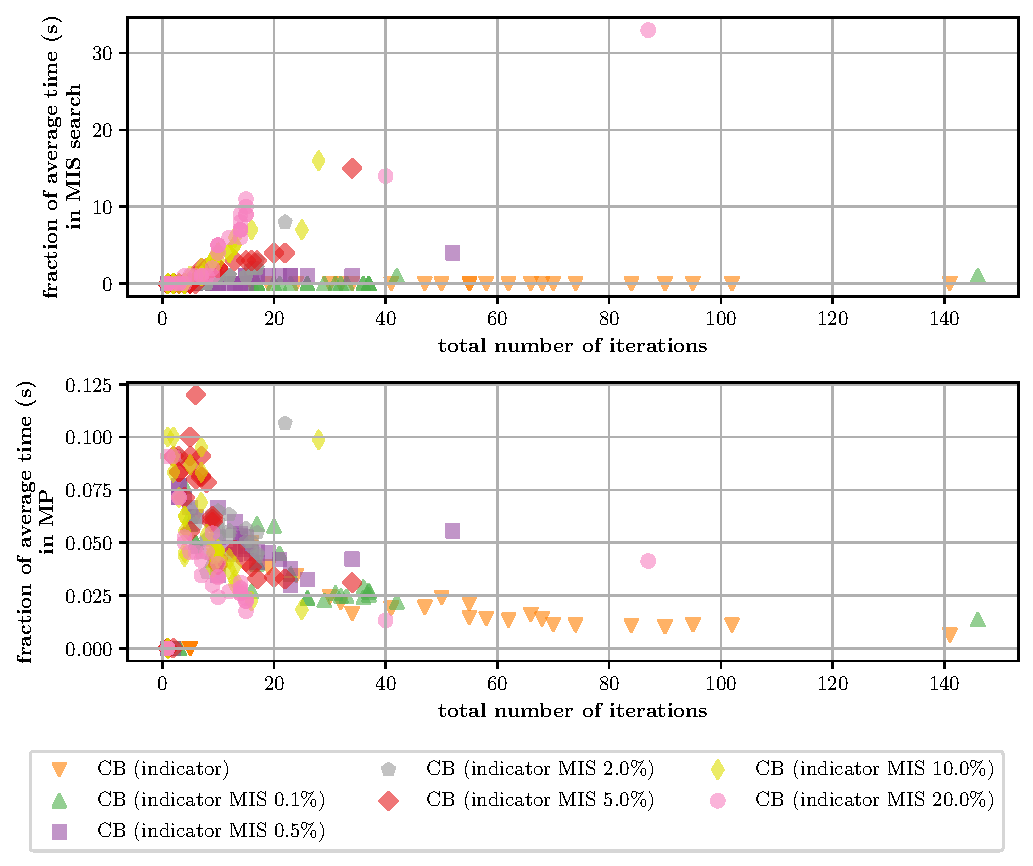
\includegraphics[width=0.8\textwidth]{Images/mis_comparison_time_vs_iterations.pdf}
    \label{fig:mis_comparison_time_vs_iterations}
\end{figure}

\begin{figure}[h!]
    \caption{solved instances by CB (big-M) and ll-FBA}
    \centering
    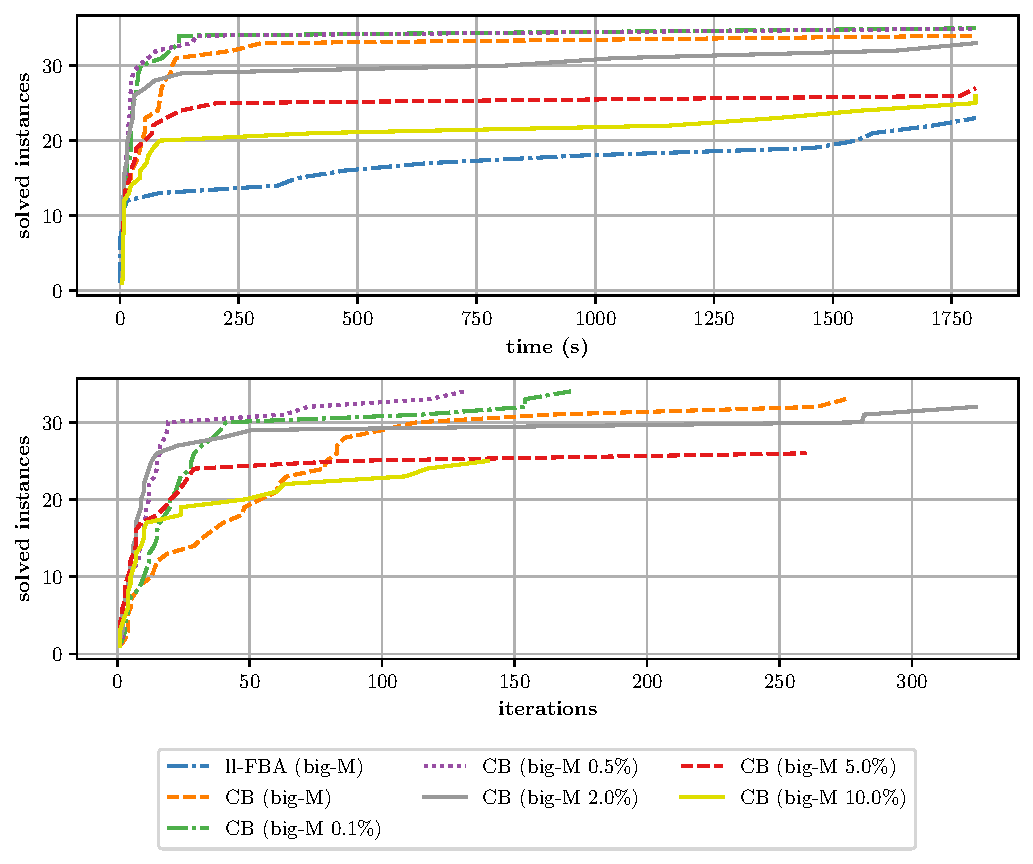
\includegraphics[width=0.8\textwidth]{Images/mis_comparison_solved_instances_big_m.pdf}
    \label{fig:mis_comparison_solved_instances_big_m}
\end{figure}
\todo[inline]{add less cuts}

\begin{figure}[h!]
    \caption{solved instances by CB (big-M) and ll-FBA}
    \centering
    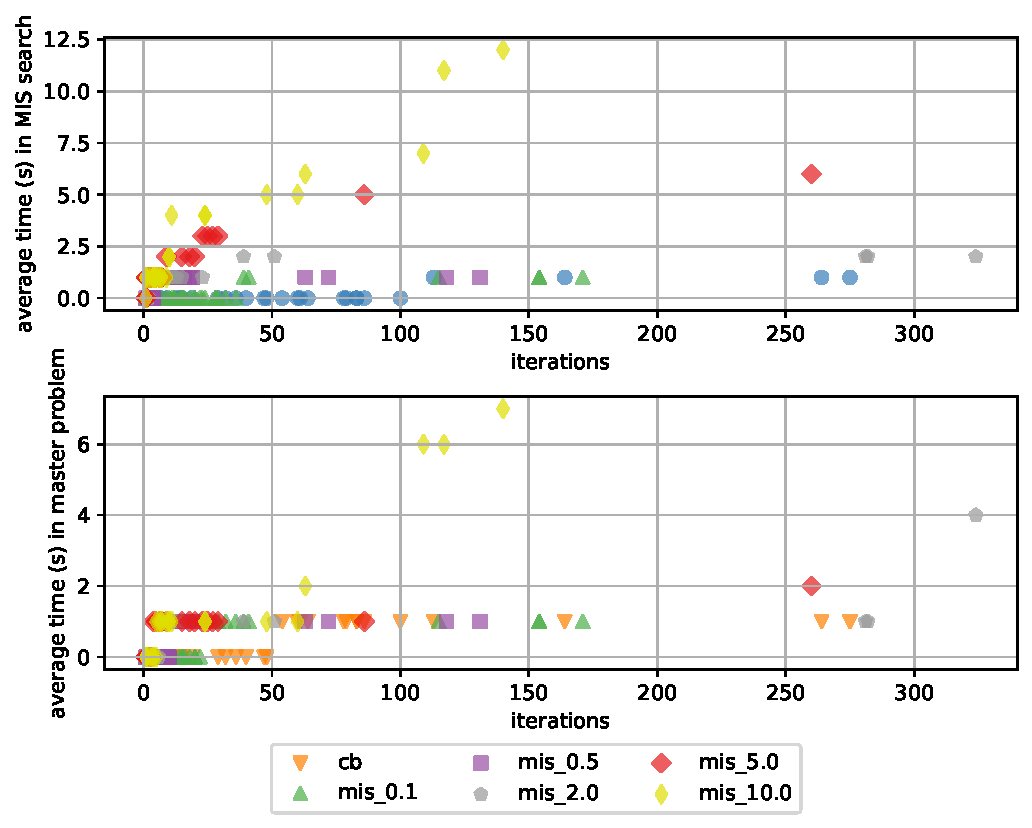
\includegraphics[width=0.8\textwidth]{Images/mis_comparison_time_vs_iterations_big_m.pdf}
    \label{fig:mis_comparison_time_vs_iterations_big_m}
\end{figure}

\begin{figure}[h!]
    \caption{solved instances by CB (big-M), CB (indicator) and CB (indicator and big-M)}
    \centering
    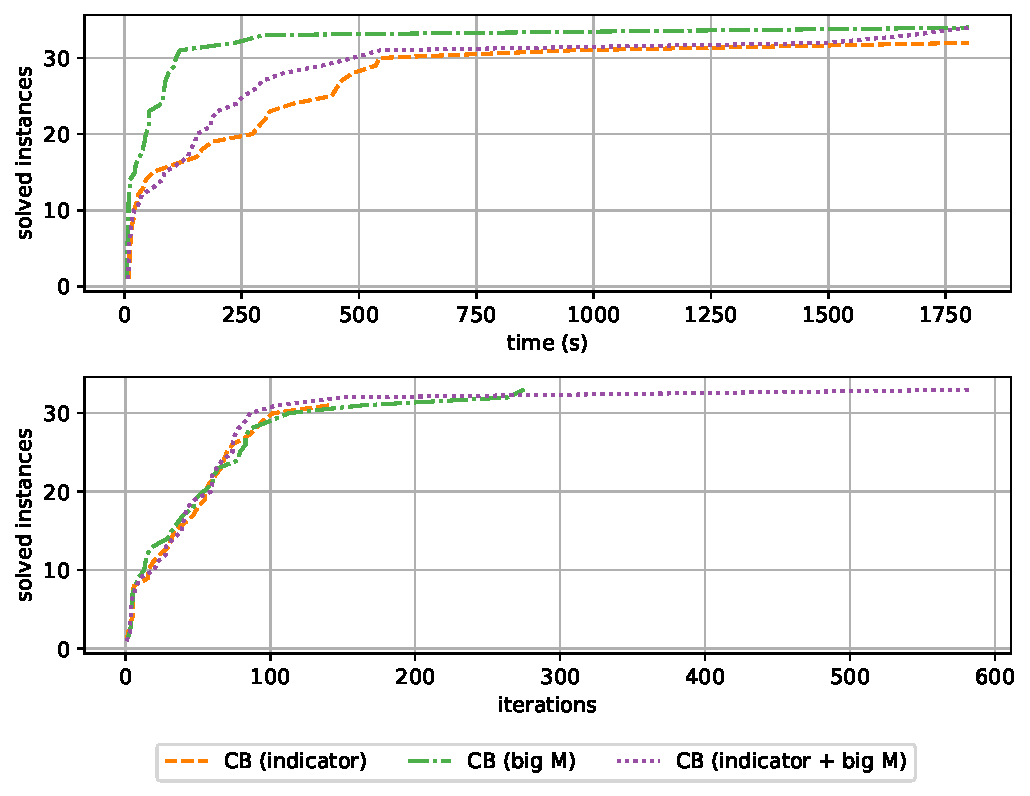
\includegraphics[width=0.8\textwidth]{Images/comparison_solved_instances_indicator_and_big_m.pdf}
    \label{fig:comparison_solved_instances_indicator_and_big_m_as_MP}
\end{figure}

\todo[inline]{note on yeast models}

\begin{figure}[h!]
    \caption{solved GECKO instances by CB (big-M), CB (big-M MIS 5\%) and ll-FBA}
    \centering
    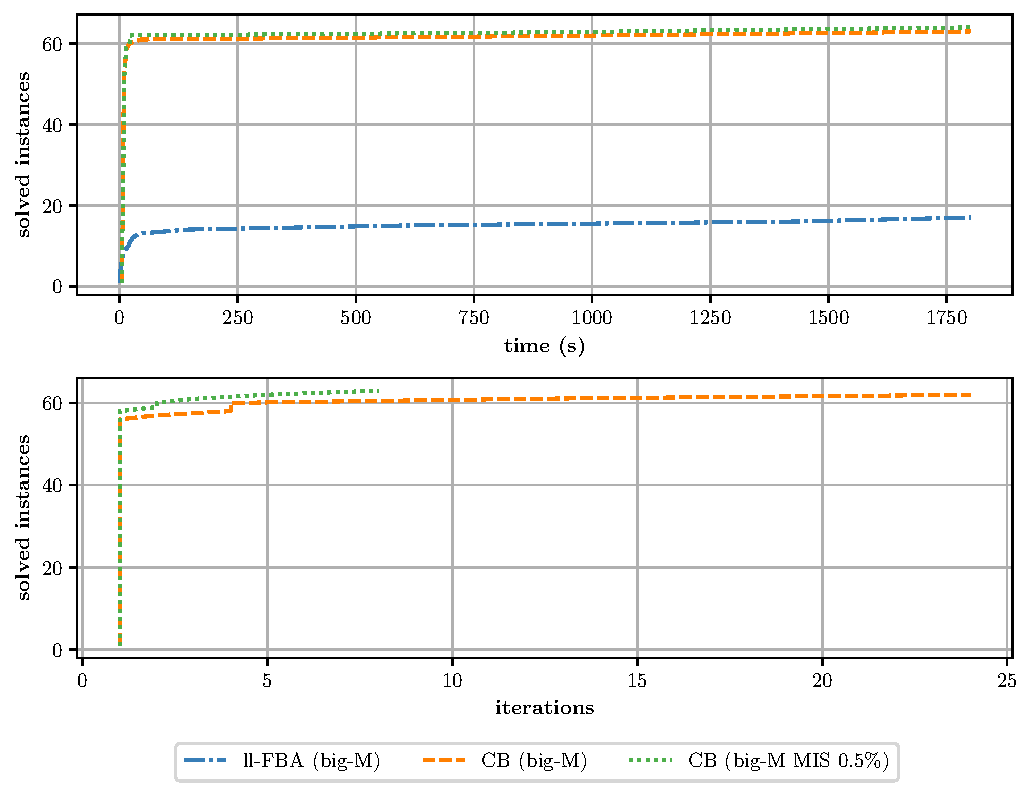
\includegraphics[width=0.8\textwidth]{Images/comparison_solved_instances_gecko_1.0e-8.pdf}
    \label{fig:comparison_gecko}
\end{figure}

\subsection{Intersection Cuts}

\subsection{Disjunctive Programming}

\begin{figure}[h!]
    \caption{solved instances by DP.jl, ll-FBA and CB}
    \centering
    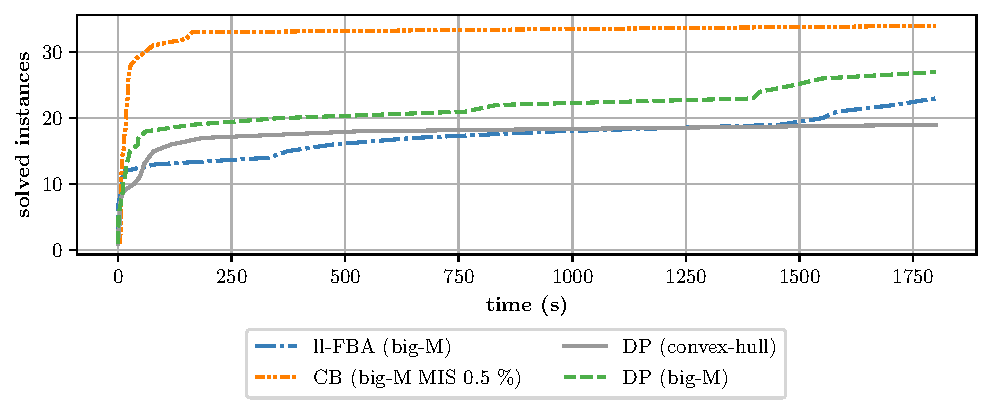
\includegraphics[width=0.8\textwidth]{Images/comparison_dp.pdf}
    \label{fig:}
\end{figure}

\todo[inline]{instances with smaller objective value are considered as NOT SOLVED, update plot}

